There are three fundamental areas of concern that make up all software systems. They are:

1. a directory structure
2. a build system
3. a version management system

They are all related, aspects of one affects aspects of each of the others.

Having a standard system makes collaborative work more efficient, especially when one needs help from others to solve a problem.

\chapter{The Packages}

There are several software components that are needed to build and use GlueX software. Most of them are assumed to be provided by the native operating system or distribution, but there are some that have to be built by the GlueX user. They are:

\begin{enumerate}
\item build\_scripts: scripts to manage building and the shell environment
\item Xerces-C: for reading XML files
\item CERNLIB: to support GEANT 3 simulations
\item ROOT: general purpose HENP toolkit
\item EVIO: CODA format data handling library
\item CCDB: Calibration Constants Database
\item JANA: event-based analysis framework
\item HDDS: detector geometry specification library 
\item sim-recon: simulation and reconstruction for GlueX
\end{enumerate}

Detailed description of these packages will not be given here; please see the GlueX Offline Software wiki page for more information.

There are in general multiple versions (releases) of each of these packages and it is often convenient to have access to more that one version of a package built and available for use. In addition some packages depend on one or several others for libraries and include files.

\chapter{The Directory Structure}

The VMS directory structure supports multiple versions of each package. For an exmple see Fig.~\ref{fig:directory-tree}. In the figure, ``gluex\_top'' is a generic name, each installation may choose a different directory name. VMS looks for the name of this directory in the environment variable {\tt GLUEX\_TOP}.

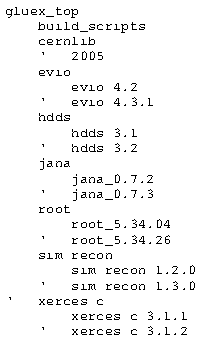
\includegraphics{tree.png}
